\ifdefined\included
\else
\documentclass[french, a4paper, 11pt, twoside, pdftex]{StyleThese}
\usepackage{iflang}
\usepackage{bibentry}



%\usepackage[sectionbib]{chapterbib}          % Cross-reference package (Natural BiB)
%\usepackage{natbib}                  % Put References at the end of each chapter
%\usepackage{bibunits}
% Do not put 'sectionbib' option here.
% Sectionbib option in 'natbib' will do.


\usepackage{fancyhdr}                    % Fancy Header and Footer

\usepackage[utf8]{inputenc}
\usepackage[T1]{fontenc}
\usepackage[french]{babel} %
\usepackage{lmodern} \normalfont %to load T1lmr.fd 
\DeclareFontShape{T1}{cmr}{b}{sc} { <-> ssub * cmr/bx/sc }{}
%\hyphenation{gar}

\usepackage{amsmath,amssymb}             % AMS Math
\usepackage{nicefrac}
\usepackage{siunitx}					%% Unites Math SI

\usepackage{blindtext}

\usepackage{datetime}

\usepackage{lipsum} 

\usepackage[inline]{enumitem}

\usepackage{hhline}
%\usepackage[left=1.5in,right=1.3in,top=1.1in,bottom=1.1in]{geometry}
\usepackage[left=1.5in,right=1.3in,top=1.1in,bottom=1.1in,includefoot,includehead,headheight=13.6pt]{geometry}

%%\renewcommand{\baselinestretch}{1.05}

%%%%%%%% Multi-figures avec sub-captions
\usepackage{caption}
\usepackage{subcaption}

% Table of contents for each chapter

\usepackage[nottoc, notlof, notlot]{tocbibind}
\usepackage[nohints]{minitoc}
\setcounter{minitocdepth}{2}
\mtcindent=15pt
% Use \minitoc where to put a table of contents

\usepackage{aecompl}

%% Package cosmetic meilleur layout du texte en jouant sur le spacing par caractères
\usepackage[activate={true,nocompatibility},final,tracking=true,kerning=true,factor=1100,stretch=10,shrink=10]{microtype}
\usepackage[absolute,overlay]{textpos} 
\setlength{\TPHorizModule}{\paperwidth}\setlength{\TPVertModule}{\paperheight}
\sloppy

%%%%%%%%%%% JOLIS TABLEAUX
\usepackage{tabularx}		%\usepackage{tabular}
\usepackage{longtable}
\usepackage{multirow}
\newcommand{\mc}{\multicolumn} 
\newcommand{\mr}[2]{\multirow{#1}{*}{#2}} 	\newcommand{\mrQ}{\multirow{-4}{*}}
\usepackage{booktabs}

\usepackage[usenames,dvipsnames]{xcolor} 

\makeatletter
\newcommand{\ccolor}[3][]{%
	\kern-\fboxsep
	\if\relax\detokenize{#1}\relax
	\expandafter\@firstoftwo
	\else
	\expandafter\@secondoftwo
	\fi
	{\colorbox{#2}}%
	{\colorbox[#1]{#2}}%
	{#3}\kern-\fboxsep
}
\makeatother

%%%%% Insertion graphiques format PGF
\usepackage{pgfplots}
\pgfplotsset{width=\linewidth, compat=1.16}%, compat=1.17}
\usepackage{adjustbox}          %%% PERMET DE LES RECADRER + FACILEMENT


%%%%%%%%%% Bullets de listes sans saut de ligne %%%%%%%%%%
\usepackage{xparse}

\ExplSyntaxOn%
\seq_new:N \l_local_enum_seq

\newcommand{\storethestuff}[1]{%
  \seq_set_from_clist:Nn \l_local_enum_seq {#1}%
}

\newcommand{\dotheenumstuff}{%
\int_zero:N \l_tmpa_int
\seq_map_inline:Nn \l_local_enum_seq {%
    \int_incr:N \l_tmpa_int% Increase the counter
    \item ##1
    % Check whether the list has reached the end -- if so, use '.' instead of ','
    %\int_compare:nNnTF 
    % { \l_tmpa_int } < {\seq_count:N \l_local_enum_seq} 
    % {,} {.}
  }
}
\ExplSyntaxOff

\NewDocumentCommand{\linebullets}{+m}{%
  \storethestuff{#1}%
  \begin{enumerate*}[label={\alph*)},font={\bfseries},itemjoin={{, }}]
    \dotheenumstuff%
  \end{enumerate*}
}

\newcommand{\cmnt}[1]{}  %%%%% AJOUT DE COMMENTAIRE MULTILIGNES


%%%%%%%%%% ECRITURE CARACTERES DANS UN CERCLE %%%%%%%%%%
%\def\circleTxt[#1]{\raisebox{.5pt}{\textcircled{\raisebox{-1pt}{#1}}}}
\newcommand{\ctxt}[1]{\raisebox{.5pt}{\textcircled{\raisebox{-1.2pt}{#1}}}}
% Glossary / list of abbreviations

\usepackage[intoc]{nomencl}
\IfLanguageName{english}{%
\renewcommand{\nomname}{Glossary}
}{ %
\renewcommand{\nomname}{Liste des Abréviations}
}

\makenomenclature

% My pdf code

\usepackage{ifpdf}

\ifpdf
  \usepackage[pdftex]{graphicx}
  \DeclareGraphicsExtensions{.pdf,PDF,.png,PNG,.jpg,JPG}
  \usepackage[pagebackref,hyperindex=true]{hyperref} %% use \autoref{} instead of Table~\ref{}.
  \usepackage{tikz}
  \usetikzlibrary{arrows,shapes,calc}
\else
  \usepackage{graphicx}
  \DeclareGraphicsExtensions{.ps,.eps}
  \usepackage[a4paper,dvipdfm,pagebackref,hyperindex=true]{hyperref}
\fi

\graphicspath{{.}{schemas/}{graphiques/}{tables/}}

%% nicer backref links. NOTE: The flag ThesisInEnglish is used to define the
% language in the back references. Read more about it in These.tex

\IfLanguageName{english}{
\renewcommand*{\backref}[1]{}
\renewcommand*{\backrefalt}[4]{%
\ifcase #1 %
(Not cited.)%
\or
(Cited in page~#2.)%
\else
(Cited in pages~#2.)%
\fi}
\renewcommand*{\backrefsep}{, }
\renewcommand*{\backreftwosep}{ and~}
\renewcommand*{\backreflastsep}{ and~}
}{
\renewcommand*{\backref}[1]{}
\renewcommand*{\backrefalt}[4]{%
\ifcase #1 %
(Non cité.)%
\or
(Cité en page~#2.)%
\else
(Cité en pages~#2.)%
\fi}
\renewcommand*{\backrefsep}{, }
\renewcommand*{\backreftwosep}{ et~}
\renewcommand*{\backreflastsep}{ et~}
}

% Links in pdf
\usepackage{color}
\definecolor{linkcol}{rgb}{0,0,0.4} 
\definecolor{citecol}{rgb}{0.5,0,0} 
\definecolor{linkcol}{rgb}{0,0,0} 
\definecolor{citecol}{rgb}{0,0,0}
% Change this to change the informations included in the pdf file

\hypersetup
{
bookmarksopen=true,
pdftitle="Prévention des fautes temporelles sur architectures multicœur pour les systèmes à criticité mixte",
pdfauthor="Daniel LOCHE", %auteur du document
pdfsubject="Thèse", %sujet du document
%pdftoolbar=false, %barre d'outils non visible
pdfmenubar=true, %barre de menu visible
pdfhighlight=/O, %effet d'un clic sur un lien hypertexte
colorlinks=true, %couleurs sur les liens hypertextes
pdfpagemode=UseNone, %aucun mode de page
%pdfpagelayout=DoublePage, %ouverture en simple page
pdffitwindow=true, %pages ouvertes entierement dans toute la fenetre
linkcolor=linkcol, %couleur des liens hypertextes internes
citecolor=citecol, %couleur des liens pour les citations
urlcolor=linkcol %couleur des liens pour les url
}

% definitions.
% -------------------

\setcounter{secnumdepth}{3}
\setcounter{tocdepth}{2}

% Some useful commands and shortcut for maths:  partial derivative and stuff

\newcommand{\pd}[2]{\frac{\partial #1}{\partial #2}}
\def\abs{\operatorname{abs}}
\def\argmax{\operatornamewithlimits{arg\,max}}
\def\argmin{\operatornamewithlimits{arg\,min}}
\def\diag{\operatorname{Diag}}
\newcommand{\eqRef}[1]{(\ref{#1})}
\newcommand{\nline}{\smallbreak\noindent}

\usepackage{rotating}                    % Sideways of figures & tables

% \usepackage{txfonts}                     % Public Times New Roman text & math font
  
%%% Fancy Header %%%%%%%%%%%%%%%%%%%%%%%%%%%%%%%%%%%%%%%%%%%%%%%%%%%%%%%%%%%%%%%%%%
% Fancy Header Style Options

\pagestyle{fancy}                       % Sets fancy header and footer
\fancyfoot{}                            % Delete current footer settings

%\renewcommand{\chaptermark}[1]{         % Lower Case Chapter marker style
%  \markboth{\chaptername\ \thechapter.\ #1}}{}} %

%\renewcommand{\sectionmark}[1]{         % Lower case Section marker style
%  \markright{\thesection.\ #1}}         %

\fancyhead[LE,RO]{\bfseries\thepage}    % Page number (boldface) in left on even
% pages and right on odd pages
\fancyhead[RE]{\bfseries\nouppercase{\leftmark}}      % Chapter in the right on even pages
\fancyhead[LO]{\bfseries\nouppercase{\rightmark}}     % Section in the left on odd pages

\let\headruleORIG\headrule
\renewcommand{\headrule}{\color{black} \headruleORIG}
\renewcommand{\headrulewidth}{1.0pt}
\usepackage{colortbl}
\arrayrulecolor{black}

\fancypagestyle{plain}{
  \fancyhead{}
  \fancyfoot{}
  \renewcommand{\headrulewidth}{0pt} %%%%%%%%%%%%%%%%%%%%%%%%%%%%%%%%%%%%%%%%%%%%%%%%%%%%%%%%%%%%%%%%%%%%%%%%%%%%%%%%%%%%%
}

%\usepackage{MyAlgorithm}
%\usepackage[noend]{MyAlgorithmic}
%\usepackage[ED=EDSYS-SystEmb, Ets=INP]{tlsflyleaf}

%%% Clear Header %%%%%%%%%%%%%%%%%%%%%%%%%%%%%%%%%%%%%%%%%%%%%%%%%%%%%%%%%%%%%%%%%%
% Clear Header Style on the Last Empty Odd pages
\makeatletter

\def\cleardoublepage{\clearpage\if@twoside \ifodd\c@page\else%
  \hbox{}%
  \thispagestyle{empty}%              % Empty header styles
  \newpage%
  \if@twocolumn\hbox{}\newpage\fi\fi\fi}

\makeatother
 
%%%%%%%%%%%%%%%%%%%%%%%%%%%%%%%%%%%%%%%%%%%%%%%%%%%%%%%%%%%%%%%%%%%%%%%%%%%%%%% 
% Prints your review date and 'Draft Version' (From Josullvn, CS, CMU)
\newcommand{\reviewtimetoday}[2]{\special{!userdict begin
    /bop-hook{gsave 20 710 translate 45 rotate 0.8 setgray
      /Times-Roman findfont 12 scalefont setfont 0 0   moveto (#1) show
      0 -12 moveto (#2) show grestore}def end}}
% You can turn on or off this option.
% \reviewtimetoday{\today}{Draft Version}
%%%%%%%%%%%%%%%%%%%%%%%%%%%%%%%%%%%%%%%%%%%%%%%%%%%%%%%%%%%%%%%%%%%%%%%%%%%%%%% 

\newenvironment{maxime}[1]
{
	\def\Arg{#1}
\vspace*{0cm}
\hfill
\begin{minipage}{0.6\textwidth}%
%\rule[0.5ex]{\textwidth}{0.1mm}\\%
\hrulefill $\:$ \\%$\:$ {\bf #1}\\
%\vspace*{-0.25cm}
\it 
}%
{%
	
\hrulefill $\:$ {\bf \Arg}
\vspace*{0.5cm}%
\end{minipage}
}

\let\minitocORIG\minitoc
\renewcommand{\minitoc}{\minitocORIG \vspace{1.5em}}

%\usepackage{slashbox}

\newenvironment{bulletList}%
{ \begin{list}%
	{$\bullet$}%
	{\setlength{\labelwidth}{25pt}%
	 \setlength{\leftmargin}{30pt}%
	 \setlength{\itemsep}{\parsep}}}%
{ \end{list} }


%%%%%%% Outils pour \comment \alert \add %%%%%
\usepackage{easyReview}
\usepackage{soulutf8} % for accented letters

\let\newalert\alert
\renewcommand{\alert}[1]{\textit{\newalert{#1}}}

%\usepackage[commandnameprefix=ifneeded]{changes} %% \chhighlight and \chcomment to avoid collision with easyReview
\renewcommand{\epsilon}{\varepsilon}

% centered page environment

\newenvironment{vcenterpage}
{\newpage\vspace*{\fill}\thispagestyle{empty}\renewcommand{\headrulewidth}{0pt}}
{\vspace*{\fill}}

\usepackage{tablefootnote}

%%%%%% MISE EN FORME CADRES DEFINITIONS/THEOREMES/LEMES %%%%%%%%%%
\usepackage{amsthm}  % for theoremstyle

\theoremstyle{plain} 
\newtheorem{theorem}{Théorème}[section]
\newtheorem{corollary}{Corolaire}[theorem]

%\theoremstyle{lemma}
%\newtheorem{lemma}[theorem]{Lemme}


\theoremstyle{definition}
\newtheorem{definition}[theorem]{Définition}


\cmnt{
	\usepackage{ntheorem} %\usepackage{amsthm}  % for theoremstyle
	%\usepackage{mdframed}
	\usepackage[most]{tcolorbox}
	
	\theoremstyle{plain} 
	\theoremindent20pt
	\theoremheaderfont{\normalfont\bfseries\hspace{-\theoremindent}}
	\newtheorem{theorem}{Théorème}[section]
	\newtheorem{corollary}{Corolaire}[theorem]
	
	\theoremstyle{plain}
	\newtheorem{lemma}[theorem]{Lemme}
	
	
	\tcolorboxenvironment{theorem}{
		blanker,
		breakable,
		before skip=\topsep,
		after skip=\topsep,
		borderline west={1pt}{10pt}{double, shorten <=12pt}
	}
	
	\theorembodyfont{\normalfont}
	\theoremindent20pt
	\theoremheaderfont{\normalfont\bfseries\hspace{-\theoremindent}}
	\newtheorem{definition}[theorem]{Définition}
	
	
	\tcolorboxenvironment{definition}{
		blanker,
		breakable,
		before skip=\topsep,
		after skip=\topsep,
		borderline west={1pt}{10pt}{shorten <=12pt}
	}
}

\cmnt{ 
	\begin{theorem}
		Ceci est un Théorème.
	\end{theorem} 
	
	\begin{corollary}
		Ceci est un Corollaire.
	\end{corollary}
	
	\begin{definition}
		Ceci est une Définition.
	\end{definition}
	
	\begin{lemma}
		Ceci est un Lemme.
	\end{lemma}
}

\def\UrlBigBreaks{\do\/\do-\do:}
\usepackage{url}

\sloppy
\begin{document}
\setcounter{chapter}{3} %% Numéro du chapitre précédent ;)
\dominitoc
\faketableofcontents
\fi

\chapter{Principe et architecture pour la gestion de fautes temporelles} \label{chap:3_PrincipeArchi}
\minitoc

In this section we describe our Monitoring and Control Agent (MCA) as a safety mechanism designed to avoid temporal faults in mixed-criticality systems. Its goal is to guarantee critical end-to-end task chain response times by avoiding interferences that could lead to such temporal fault.

The MCA role is first to monitor the state of a HI-criticality task chain to detect potential deadline miss. If such a potential fault is anticipated, then the MCA switches the system to HI-criticality mode, pausing all non essential workload (LO-criticality tasks), to prevent further interference on the HI-criticality tasks and allow a safe termination. To be efficient, the switch  must be triggered only when necessary (as a “mode switch procrastination”, as called in~\cite{hu_ffob_2019}). That is why we also focus on end-to-end deadline, rather than individual task deadlines, in order to avoid false-positive switching, meaning switching to HI-criticality mode although there is slack in the task chain. Indeed, with an end-to-end perspective, we can use the slack given by a task finishing early to compensate the lateness of an other task in the chain.

In the following, we introduce the execution model considered in our work, then we describe the proposed MCA architecture to finally present in more details the principle of the anticipation mechanism.

\section{Un modèle basé sur des chaînes de tâches pour garantir les contraintes temporelles}

    %The model describes how HI-criticality tasks behave and are linked in a chain to produce a HI-criticality functionality. Note that this model is one among many usable with our approach. We choose this one for ease of presentation. 
    
    Afin d'étudier et développer notre mécanisme de gestion de fautes temporelles dans le cadre d'un système à criticité mixte, nous avons besoin de formaliser la façon de représenter les tâches qui seront à l'étude et leur modèle. Il est à noté que le modèle ici proposé est relativement arbitraire et choisi essentiellement pour des raisons de commodité. De fait, on retiendra deux critères principaux pour guider le choix de notre modèle~: la simplicité d'implémentation et l'accessibilité à des suites logicielles qui peuvent servir de tâches pour simuler un système réel lors de nos tests. L'objectif est ainsi de trouver un juste milieu entre un modèle représentatif d'une réalité technique dans les milieux industriels d'une part, et un modèle qui nous évite des surcoûts de développement pour obtenir une première preuve de concept fonctionnelle.
    
    
    Ce modèle doit décrire d'une part la méthode d'exécution des tâches, la façon d'interagir, entre-elles, notamment pour les tâches à haut niveau de criticité qui sont reliées sous la forme d'une chaîne pour réaliser une fonction critique. Il est à noter que le mécanisme de sûreté de fonctionnement que nous proposons par la suite est \textit{in fine} indépendant du modèle de tâche ici proposé. Il conviendra d'adapter au besoin la partie de Contrôle du mécanisme, de façon à ce que son exécution prenne en compte l'état d'exécution du système selon le modèle de tâche utilisé, s'il est différent de celui présenté ici. Typiquement la vérification des contraintes de précédence peut différer. On aura l'occasion d'aborder rapidement ces aspects par la suite, avec quelques exemples de modifications requises suivant des changements de ce modèle de tâche. \alert{A voir...}
    
    \subsection{Modèle de tâches}
        \alert{Il manque ici la présentation/définition de "système à criticité mixte" ainsi que ce que l'on va nommer tâches critiques"/"non critiques".  A voir comment séparer cela de la partie "cas d'application industrielle".... }

    Le système ici étudié est dit à niveau de criticité dual. Il exécute un set de tâches logicielles (dite "charge utile") exécutées sur un support logiciel (classiquement, le système d'exploitation). Elles se répartissent entre les tâches à haute criticité d'une part ("tâches critiques"), et à faible criticité d'autre part (non critiques). \textit{c'est la partie à étendre.}
    
    La plupart des hypothèses faites ici se focalisent sur les tâches critiques, tandis que la seule hypothèse forte sur les tâches non critique est la capacité à les stopper (soit un arrêt total soit une mise en pause) et relancer en cours d'exécution. Sous les systèmes type Unix, cela correspond typiquement à l'envoi d'un signal SIGSTOP et SIGCONT. Sans cette condition, les notions de mode nominal et de passage en mode dégradé ne sont pas exploitables pour notre besoin. 
    Chaque tâche critique $\tau_i$ est activée et exécutée suivant une période $T_i$. A chaque période, le \textit{job} $\tau_{i,j}$ correspond à la $j^{ieme}$ exécution de la tâche $\tau_i$. On peut alors noter pour chaque job $\tau_{i,j}$ son moment d'activation $a_{i,j}$, son début d'exécution $s_{i,j}$ et sa terminaison $e_{i,j}$. On considère qu'un job consomme toutes ses données d'entrée (inputs) au début de son exécution, s'exécute et fourni à la fin de son exécution les données de sortie. Les données d'entrée et de sortie des tâches sont stockées en espace mémoire partagé : la transmission des données d'une tâche à l'autre se fait de façon asynchrone.
    Cela nous mène à la question de l'interaction entre les tâches et notamment la façon de représenter la précédence.

    \subsection{Modèle de Chaînes de Tâches}
    
    \textit{Il faudrait commencer par nommer différents modèles d'exécution de tâches existants ici, c.f. ~\cite{friese_estimating_2018}}
    La question de la dépendance entre les tâches est importante pour aborder le problème des contraintes temps-réel avec une vision plus macroscopique. En effet dans le cadre de l'usage de tâches ayant des contraintes temporelles "molles" (soft real-time), c'est uniquement avec une vision plus globale de l'exécution du système qu'il est possible de tirer au maximum parti des légers dépassements pour éviter dans la globalité d'avoir recours à des politiques d'exécution des tâches plus restrictives, et par conséquent qui sous-exploitent la puissance de calcul disponible.
    Nous considérons ici la dépendance entre les tâches via les données partagées entre ces dernières selon un modèle type producteurs/consommateurs. Les tâches ont des relations de cause à effet et par conséquent, d'un point de vue strictement fonctionnel on peut décrire le système comme étant une accumulation de fonctionnalités réalisées par l'exécution de tâches successives. Cela permet alors d'introduire la notion de contrainte temporelle fonctionnelle, qui décrivent des contraintes d'exécution de chaînes de tâches bout-en-bout.
    
    
    On représente une dépendance entre tâches sous la forme de chaînes de tâches, suivant le modèle $\tau_{1} \rightarrow \tau_2 \ldots \rightarrow \tau_n$. Dans un tel exemple, $\tau_1$ est la \textbf{tâche d'entrée} de la chaîne, tandis que $\tau_n$ est la \textbf{tâche de sortie} de la chaîne. Notons que ce modèle peut être étendu pour supporter des tâches représentées par un Diagramme Orienté Acyclique (Directed Acyclic Graph - DAG) sans difficulté. Nous nous contentons ici de travailler avec des chaînes directes, sans divergences ou convergences dans le graphe. De fait, cet ajout de complexité dans le modèle de chaîne de tâche n'apporte rien sur les résultats et la globalité de la démarche et ne demande, au demeurant, pas de modifications sur la solution proposée. 
    
    \textit{J'hésite à présenter ça dans "l'autre sens" : présenter un modèle de chaînes de tâches plus complet (avec div/conv etc.) et au final restreindre le modèle à des chaînes linéaires qu'au niveau du cas d'étude (chapitre 5)}
     
    Dans ce contexte, on peut donc définir la relation entre une tâche $\tau_i$ et son successeur $\tau_{i+1}$. Pour produire la donnée de sortie du job $\tau_{i+1,k}$ de la tâche $\tau_{i+1}$, ce dernier consommes toutes les données d'entrée en attente provenant des jobs $\tau_{i,j}$. Les données en attente étant celles qui n'ont pas été consommé par le job précédent de $\tau_{i+1}$, i.e. $\tau_{i+1,k-1}$. On peut donc écrire que pour un $i,k$ donnés, sont consommés les données de tous les jobs $\tau_{i,j}$ ssi $j \textup{ tel que } e_{i,j} \leq s_{i+1, k}$ et $s_{i,j} > e_{i+1, k-1}$. Autrement dit, un job $\tau_{i,j}$ n'a un effet sur $\tau_{i+1,k}$ si et seulement si ce dernier est le premier job de $\tau_{i+1}$ exécuté après la terminaison de $\tau_{i,j}$.

    %%i.e. un job $k$ donné de la tâche $i+1$ consomme toutes les données des jobs de la tâche $i$ qui se sont terminées avant le début de son exécution et qui n'ont pas été consommées par le job précédent $k-1$.
    
    Dans ces conditions là, on nomme $\tau_{i+1,k}$ le \textbf{successeur} du job $\tau_{i,j}$. On note $succ()$ la fonction qui permet de trouver le successeur d'un job donné. Par extension, la fonction itérative $succ^{n-1}()$ permet de trouver le job de sortie d'une chaîne de tâche donnée, selon le job d'entrée. 
    Pour illustrer cela, on peut prendre l'exemple d'une chaîne de trois tâches $\tau_1 \rightarrow \tau_2 \rightarrow \tau_3$, tel que représenté en~\autoref{fig:chain_chronogram}. On peut noter que une des exécutions de la chaîne de tâche, débutant par $\tau_{1,1}$, donne : $succ^{2}(\tau_{1,1}) = succ(succ(\tau_{1,1})) = succ(\tau_{2,2}) = \tau_{3,2}$. %On a alors le temps de réponse de la-dite chaîne : $R_1 = e_{3,2} - s_{1,1} = 31 - 5 = 26$ unités de temps.


    \begin{figure}[ht]
        \centering
        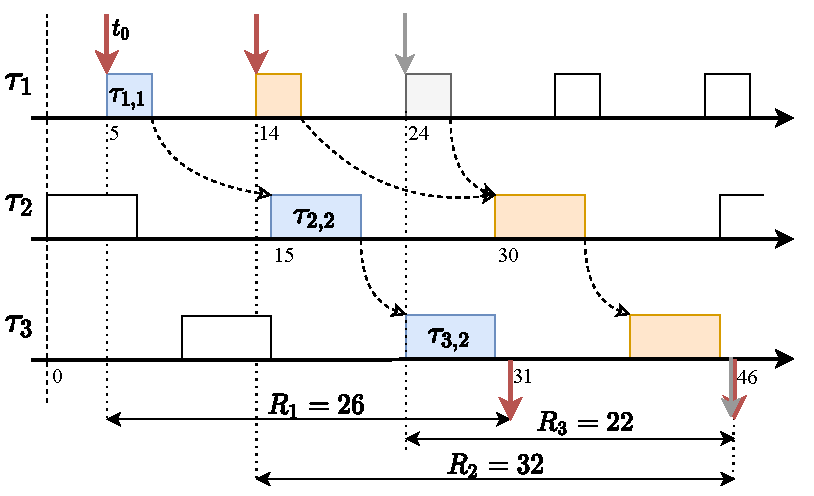
\includegraphics[width=.8\linewidth]{TaskChain_chronogram.pdf}
        \caption{Task chain run-time example with $\tau_1 \rightarrow \tau_2 \rightarrow \tau_3$}
        \label{fig:chain_chronogram}
    \end{figure}
        
    %%\subsection{Contrainte bout-en-bout de la chaîne de tâche}
    The notion of successor allows the definition of the response time of the chain: it is the elapsed time between the activation of an \emph{entry} task job $\tau_{1, j}$ and the end of the \emph{exit} task job $\tau_{n, k} = succ^{n-1}(\tau_{1, j})$. Noting $R_{j}$ the response time of this activation, we have $R_{j} = e_{n,k} - a_{1,j}$. On \autoref{fig:chain_chronogram} the resulting response times $R_1$, $R_2$, $R_3$ of the first three entry task activation of the chain are represented. 
    Note that with this definition, because tasks can have different periods, several jobs of $\tau_i$ can have an effect on a job of $\tau_{i+1}$, as shown in \autoref{fig:chain_chronogram} 

    Intuitively, an \textbf{end-to-end deadline} means that the time it takes for an input of the chain to have an effect on its output, i.e. its response time, must be bounded. Thus, given a deadline $D$, to be temporally safe our task chain must satisfy: $\max_{j \in \mathbb{N}}\{R_j\} \leq D$. 
    %Thus, in our model it means that the elapsed time between the activation of an \emph{entry} task job $\tau_{1, j}$ the end of the \emph{exit} task job $\tau_{n, k}$ which depends on $\tau_{1, j}$ must never exceed a given value $D$.
    
\section{Principe de mécanisme d'anticipation - structure Moniteur \& Commande}
    \subsection{Méthode d'anticipation}
    
    Our anticipation mechanism is based on the run-time monitoring of the task chain progress. To that end, we introduce the notions of \textbf{Task Chain State} and \textbf{Task Chain Execution Trace} (TCET). A TCET contains an entry task job and all the iterative successors of that job. At a time $t$ a TCET can be \emph{active}, if its entry task job has been activated and if its exit task job has not yet ended, or \emph{inactive} otherwise. 
    At time $t$, the \textbf{Task Chain State} is defined as $S(t)=\langle t_0, \tau_i\rangle$ with $t_0$ the oldest activation among active TCET, and $\tau_i$ the next task from this TCET to be executed. This way the task chain state indicates the remaining tasks to be executed on the chain and its current response time. Having an estimation of the \emph{remaining Worst Case Response Time} ($rWCRT(\tau_i)$) at that moment for this TCET, the anticipation mechanism can figure out if we are running into a potential deadline miss. For instance, at $t=18$ on \autoref{fig:rwcrt_chronogram}, the task chain state would be $S(t)=\langle 5, \tau_{2} \rangle $. With this $S(t)$ at a given time t, we have the current chain response time $RT(t) = t - t_0$ and the remaining response time $rWCRT(\tau_i)$ estimation (i.e. $\tau_2 \rightarrow \tau_3$ remaining) to check if the execution can finish in time.

    \begin{figure}
        \centering 
        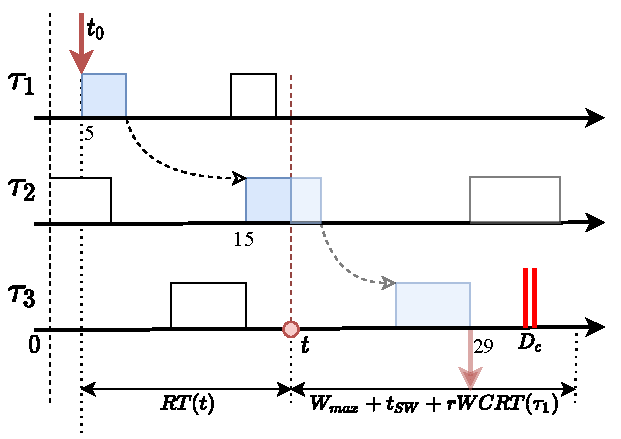
\includegraphics[width=.8\linewidth]{rWCRT_chronogram.pdf}
        \caption{active Task Chain Execution Trace with computed anticipation example}
        \label{fig:rwcrt_chronogram}
    \end{figure}
    
    Obviously, the estimation of $rWCRT(\tau_i)$ is an important element of the approach. It can be done either experimentally or analytically. We choose an experimental approach for our experiments as the analytical approach is intractable for complex application on a modern multi-core processor or would imply an overly pessimistic estimation. Details of the experimental protocol used for this estimation is given in section~\ref{protocol}. %compared to a probabilistic approach. 
    This estimation is made during system integration, without the LO-criticality tasks, thus $rWCRT(\tau_i)$ estimates the worst case time remaining before the end of the task chain if executed in HI-criticality mode. 

    To decide if it is safe to continue in LO-criticality mode, the anticipation mechanism periodically checks the task chain state. Each observation at a time $t$ is considered temporally safe if the following inequality (adapted from \cite{kritikakou_run-time_2014}) holds:
                \begin{equation} \label{safe_cond}
                RT(t) + rWCRT(\tau_i) + W_{max} + t_{SW} \leq D
                \end{equation} 
                 
    where $W_{max}$ is the worst time between each observations and $t_{SW}$ the latency to switch to the HI-criticality mode. Let us assume that (\ref{safe_cond}) holds, we show that it is safe to wait for the next observation to decide if there is a need to switch. Let $t_{next}$ the time of the next observation. 
    By definition, $t_{next} \leq t + W_{max}$ then necessarily $RT(t_{next}) \leq RT(t) + W_{max}$, thus  \\$RT(t_{next}) + rWCRT(\tau_i) + t_{SW} \leq RT(t) + rWCRT(\tau_i) + W_{max} + t_{SW}$. 
    Also, $rWCRT()$ can only decrease as time passes, so $rWCRT(t_{next}) \leq rWCRT(\tau_i)$ and $RT(t_{next}) + rWCRT(t_{next}) + t_{SW} \leq RT(t) + rWCRT(\tau_i) + W_{max} + t_{SW}$. 
    Since (\ref{safe_cond}) holds, we have $RT(t_{next}) + rWCRT(t_{next}) + t_{SW} \leq D$. 

    Hence, it will be safe to switch to LO-criticality mode at the next observation. The setting of the $W_{max}$ parameter is discussed in the next section.

Most of our architectural choices have been made to facilitate portability and deployment of our solution. To that end, the MCA intervenes on the task at the highest level possible and does not require alteration of tasks code or binary.

To help with the estimation of $rWCRT$, we assume that the HI-criticality task chain execute on a single core. To avoid interference between the MCA and the task chain we prevent the MCA to use the same core. Lo-criticality tasks can execute on any core as depicted on \autoref{fig:SoftwareArchitecture}. 

\begin{figure}[ht]
            \centering
            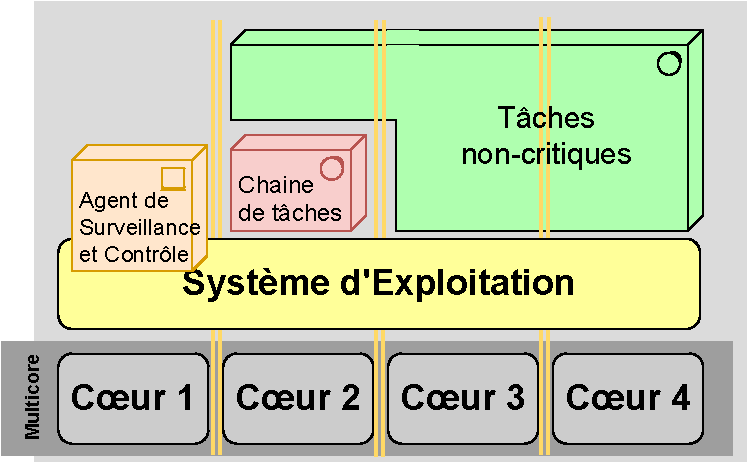
\includegraphics[width=.7\linewidth]{ArchitectureLogicielle.pdf}
            \caption{Monitoring \& Control Agent basic concept} \label{fig:SoftwareArchitecture}
\end{figure}

      The Monitoring and Control Agent is made of two components: a \emph{Task Wrapper Component} and a \emph{Core Control Component} as shown in \autoref{fig:architecture}.
        \begin{figure}[ht]
            \centering
            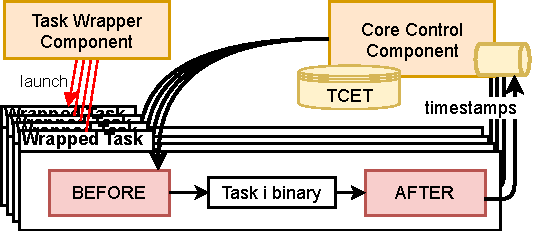
\includegraphics[width=0.85\linewidth]{ArchitectureFramework.pdf}
            \caption{Monitoring \& Control Agent Architecture\label{fig:architecture}}
        \end{figure}
        
        
        \subsubsection{Task Wrapper Component (TWC)} It is responsible for encapsulating the system tasks between two software wrappers, ``Before" and ``After". Those wrappers have two roles: \begin{itemize}
                \item provide timestamps (start and end of HI tasks) to the Core Control Component.
                \item prevent LO tasks execution in HI-criticality mode.
            \end{itemize}
            
%%%%%%%%%%%%%%%%%%%%%%%%%%%%%%%%%%%%

        The timestamps are queued to be processed by the Core Control Component to update the TCET.
        The ``Before" wrapper is also used to prevent LO task execution in degraded mode. There is no need for an ``After" wrapper for LO tasks.

        \subsubsection{Core Control Component (CCC)}
           The Core Control Component executes with a period $T_{ccc}$. It updates each \textbf{active Task Chain Execution Trace} (TCET), taking into account timestamps received since its last execution and compute the task chain state $S(t)$, enabling the evaluation of $RT(t)$ and $rWCRT(\tau_i)$. Then CCC checks if inequality~(\ref{safe_cond}) is still true. If not, the CCC switches to degraded mode to guarantee the task chain deadline. The mode switch is realised through two actions: sending a Pause signal to every LO-criticality tasks, and signaling ``Before" wrapper to prevent any new execution.
        
\cmnt{
            The Core Control Component stores each active \textbf{Task Chain Execution Trace} (TCET) in order to compute the task chain state $S(t)$ at any time.
            
            %The Core Control Component updates the task chain timing state periodically to check if the deadline can still be guaranteed. The $S(t)$ update frequency is fixed and not directly triggered by a monitoring message (i.e. at one update we could have multiple pending finished tasks to consider or none). Consequently, such period must be chosen regarding the tasks' execution times to avoid having too much monitoring messages to take into account. 
            Task chain state updates are triggered periodically, every $T_{ccc}$, and not asynchronously (for each new monitoring message) to avoid being dependent on when the ``Before" and ``After" wrapper are executed. This way we can still decide to switch to degraded mode as ET(t) still increases as we are getting closer to the deadline even with no new monitoring message.
            
            At each TCET update, the CCC check if inequality~\ref{safe_cond} is still true. If not, the CCC switches to degraded mode to guarantee the task chain deadline. The mode switch is made first by sending a Pause signal to every non-critical task from the CCC, in addition to the TWC blocking feature mentioned above.
        }
        
            The CCC parameters $t_{sw}$ and $W_{max}$ are important to define. If those parameters are underestimated, then it is not safe to use inequality~(\ref{safe_cond}). We estimate them for our experimental platform in \ref{expe_calibPhase}. 
            $W_{max}$ is the maximum duration between two CCC checkpoints. It is directly dependent to the CCC period $T_{ccc}$. If Hi-criticality tasks are periodic, which is typical, it is simple to set this value, around the smallest task period. This way we have the guarantee of not overflowing the timestamps queue used by the CCC. A greater value is possible, but we must take care to process the $TCET$ updates faster than the arrival of timestamps. For other tasks activation models, we must identify the highest task timestamps arrival rate to avoid any queue overflow. 
            It is also important to set $T_{ccc}$ --and thus, $W_{max}$-- as it will directly influence the sensitivity of our anticipation mechanism. With a higher CCC update frequency --and consequently a lower $W_{max}$-- we switch to degraded mode later. Also, it will naturally use more computing resources. A higher value triggers sooner and may increase the number of unneeded switches to degraded mode (i.e. false positives). 
            %Future work could aim at measuring more precisely $W_{max}$ influence. 

        \cmnt{
            One should note that what makes such approach possible is the evolution of the $rWCRT$ at run-time and as the $S(t)$ evolves. It would not be possible to apply such approach when it comes to monitor \& control individual tasks to guarantee their individual deadlines. For individual deadlines, our method would fit only if we are able to monitor tasks timing state ``inside" the tasks execution, i.e. instrumenting the tasks source code to add internal checkpoints. Such approach on individual tasks would discard by definition the use of black box software assumption for instance, and otherwise would need much higher refresh rate frequencies in order to follow individual tasks execution timing state. Such solution is presented for individual tasks in~\cite{kritikakou_dynascore_2017}.
            }
            
    \subsection{Mode dégradé et tâches non vitales}
    \subsection{Méthode de recouvrement}
    \subsection{structure en Moniteur + Commande - Architecture Logicielle}
\section{Application au domaine  automobile (diag. fonctionnel, SWC, etc)}
    \subsection{Concept Description}
        Our approach presents a software execution \emph{Monitoring and Control Agent (MCA)} to guarantee end-to-end deadline constraints.
        %Our challenge is to investigate that an appropriate combination of general-purpose scheduling policies, tasks allocation to cores, freezing strategies of non-critical tasks when critical tasks need more computing resources is a solution to comply with end-to-end real-time constraints. %In practice deadline specifications are often arbitrary and approximate due to system complexity. 
        We focus on the respect of end-to-end constraints of tasks chains, not individual tasks constraints. The idea behind this is to offer more ``flexibility'' on tasks scheduling for guaranteeing mandatory task chains constraints if we control only end-to-end constraints instead of every critical task timing constraint. By doing so, we gain "flexibility" as we allow some parts of the chain to be behind time as they can be compensated before the end of the chain without any external action. The MCA monitors at run-time the execution time of critical tasks and anticipate when the end-to-end deadlines may be compromised to stop non-critical tasks when needed in order to avoid such risk. The anticipation is based on the estimation of remaining WCET. Finally, when the critical task chain recovers from the potential risk, the non-critical tasks can resume their execution to get back to a nominal state.
        
        We define a \textit{degraded mode}, opposed to the \textit{nominal mode} of execution. In nominal mode, critical and non-critical tasks are executed normally. In Degraded mode, non-critical tasks are not executed, to prevent further interferences on critical tasks. The degraded mode implies simpler WCET estimations because we eliminate the disturbances from non-critical tasks; such WCET will be lower than in a nominal mode. It is probably less pessimistic as we eliminate memory interferences, non-critical tasks scheduling and possible common resources (drivers for instance) usage. The main disturbances remaining will be only between the tasks from the chain. Consequently, our anticipation mechanism will be based on reduced estimation of WCET (compared to nominal mode), to activate degraded mode only as a last resort.
        \smallbreak
        To reach degraded mode, MCA role is to pause/stop non-critical tasks execution. This control is triggered by an anticipation algorithm. To be efficient, this algorithm should trigger the control at the latest possible time while guaranteeing real-time end-to-end constraints.
        
        %Individual deadline could be compromised however the goal is to respect task chains deadlines.
        %Individual WCET are also useful, but if they are not available, approximations extracted from behavioral models are enough, for example with an equal distribution of the global end-to-end time value as described in [ref].  
        \begin{figure}[h]
            \centering
            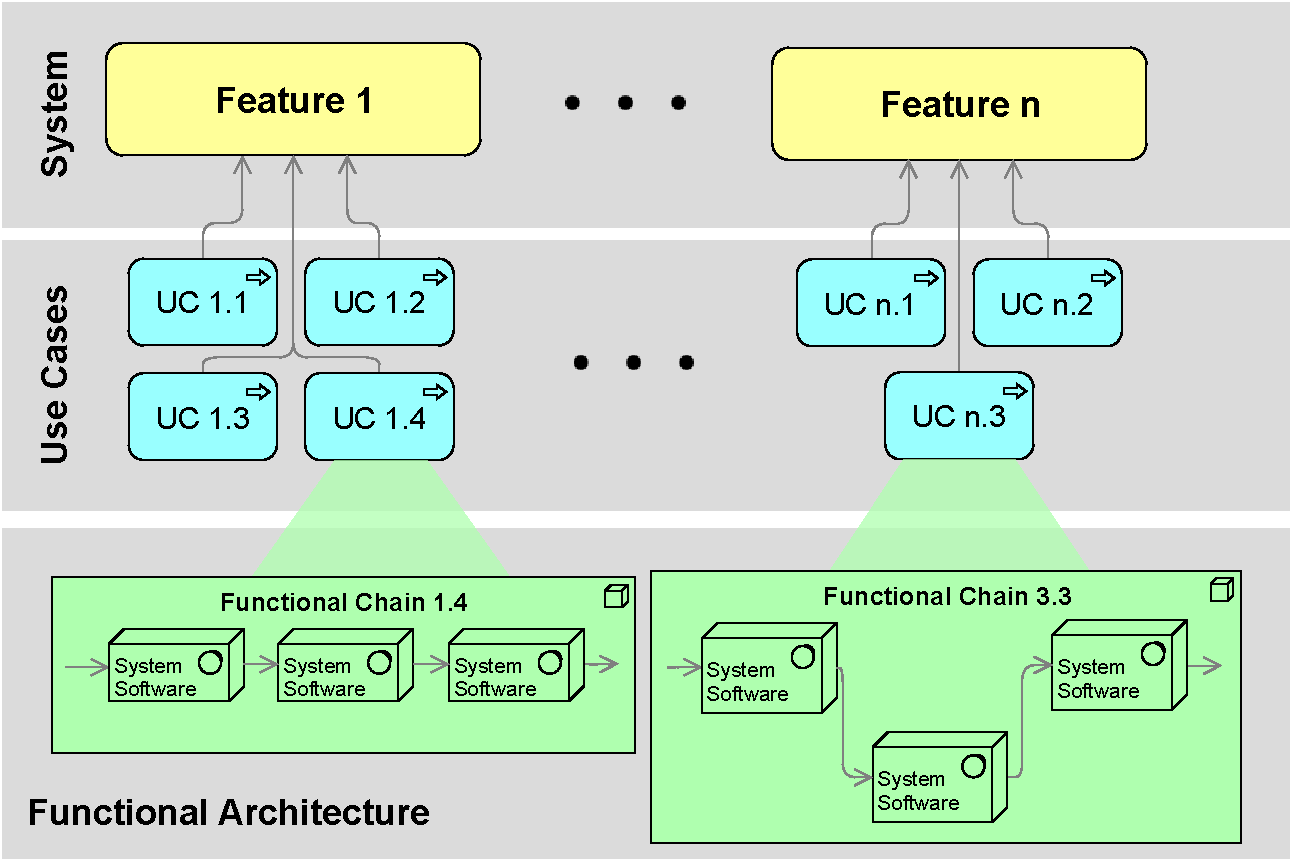
\includegraphics[width=\linewidth]{SchemaChaineFonctionnelle}
            \caption{Functional Architecture definition} \label{fig:funcArch}
        \end{figure}
        \smallbreak
        \subsubsection{Functional Specification} 
            A critical task chain must describe the implementation of a system functionality from its triggering to its consequence. This would stick most of the time with a computing chain going from a sensor measure to an actuator command. First idea would be to stick with safety criticality levels (ASIL D to ASIL A and QM, for automotive applications), but we quickly notice that there is no direct link between this classification and critical tasks chains. A safety critical task is not necessarily defined from its timing constraints. The only possible conclusion here is that a critical task chain only includes non-QM tasks. 
            \smallbreak
            We propose here a definition based around high-level specifications as represented in figure~\ref{fig:funcArch}. The global system is defined as a set of features\footnote{Features: all the services the system must provide. e.g: Lane Support System (LSS) is a feature.}. Every feature gathers a set of functionalities that are translated into Use Cases\footnote{e.g: Lane Departure Warning \& Lane Keeping Assist are part of the use cases of LSS feature.}. A Use Case defines a feature behavior for a given context and inputs (and the consequent outputs). Finally, those are translated into functional chains representing different functions and their interactions needed for the realization of the Use Case. 
            
            If we combine this information with a severity classification in case of failure of the use cases, it is possible to define critical chains as functional chains with a high severity risk. This is one possible criterion allowing an easy separation between a critical functional chain and the others. It could be adapted during the design phase, depending on the functional chains allocated to the processor. 
            \smallbreak
            Such information allows to define the software components involved in the critical task chain. All the software components used to realize a critical functional chain form a critical task chain at an OS point of view. At this point, it is possible to define the task chain end-to-end deadline, following the severity temporal risk in case of failure. Such deadline should be at minimum the sum of individual tasks deadline, but could probably be higher, depending on the global system and the task chain function. Our objective is to guarantee such critical task chain end-to-end execution time on the multicore.
\ifdefined\included
\else
\bibliographystyle{StyleThese}
\bibliography{these}
\end{document}
\fi
